\subsection{Baseline Models}
\label{sec:baselines}
As no other research provides a baseline that can be compared to for this system, I propose two baseline controllers: a differential controller based on the constant curvature assumption and a PID controller based on a prismatic joint assumption. The selection of the constant curvature model is motivated by its ease of derivation and implementation. Other models, such as those based on a variable curvature backbone representation may provide more accurate results than our selected baseline at the expense of increased computation \cite{10.3389/frobt.2020.630245}. These models also have their own challenges representing the dynamic effects of continuum robots. Future works may look at the results of these models on this system but it is deemed as beyond the scope of this thesis. The PID controller was chosen as it is a fast model both in runtime and implementation time, and can be tuned to work reasonably well in a closed-loop scenario.  

\subsubsection{Robot Model}
First, a robot model is developed that maps an arm's curvature value to a tendon displacement. Equation \eqref{eq:ik_ktoq} solves for the change of tendon length required to achieve a given constant curvature. Two solutions are provided, one for each side of the beam. Equation \eqref{eq:ik_ktoq} is used to find the tendon length given a beam's curvature, assuming a fully constrained tendon path \cite{10.3389/frobt.2020.630245} along the length of the beam. 

\begin{equation}\label{eq:ik_ktoq}
    \Delta l_{t,i} = \pm\ell_i\ell_t\kappa_i
\end{equation}

Equation \eqref{eq:ik_ktoq} can be extended to consider the prototype motor's gear ratio and spindle radius which the tendons are wrapped around. This gives an expression for the motor rotation required to achieve the desired tendon length displacement. The motor rotation $q$ found in Equation \eqref{eq:joint} is the joint variable for the proposed PCR. I take the positive solution as both tendons are actuated in their respective directions by the same motor. 

% Joint variable calculation 
\begin{equation}\label{eq:joint}
    q = \kappa G \ell_i \frac{\ell_t}{r_m}
\end{equation}

\subsubsection{Constant Curvature Controller}
A model using the constant curvature assumption \cite{doi:10.1177/0278364910368147} is used as a baseline model for this parallel continuum robot. This model is used to solve the inverse kinematic problem. This is used to determine control signals for the robot during the data generation, enabling the ability to control the position of the end effector (with some error). Equation \eqref{eq:cc/ik} gives a general expression relating the curvature of a constant curvature beam and a beam's base and end position \cite{slilge_2020}. 

\begin{figure}[H]
    \centering
    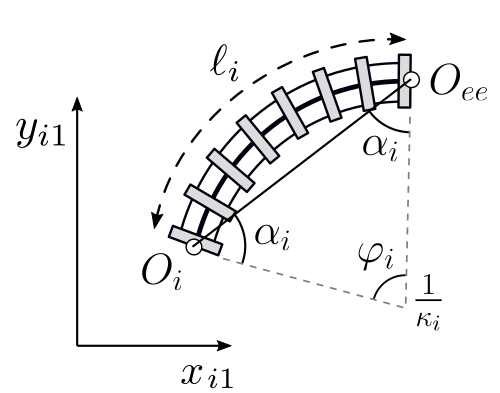
\includegraphics[width=0.6\textwidth]{images/constant_curvature_link.png}
    \caption{Constant curvature model diagram}
    \label{fig:cc_controller}
\end{figure}

% Inverse Kinematic Equation
\begin{align*}
|| O_{ee} - O_i || &= 2\frac{1}{\kappa_i}\cos(\alpha_i) \\
&= 2\frac{1}{\kappa_i}\sin\left(\frac{\varphi_i}{2}\right)\\
h(\kappa_i, O_{ee}) = h_i = 0 &= \frac{2}{\ell_i\kappa_i} \sin\left(\frac{\ell_i\kappa_i}{2}\right) - \frac{|| O_{ee} - O_i ||}{\ell_i}\stepcounter{equation}\tag{\theequation}\label{eq:cc/ik}
\end{align*}

The solution for $\kappa$ is found by finding the roots of Equation \eqref{eq:cc/ik}. For the parallel continuum case, one solves Equation \eqref{eq:cc/ik} for each of the robot's arms. One extra check is required that the target point is within reach of each arm to guarantee a solution. The solution is found numerically using scipy.optim.fsolve\footnote{\url{https://github.com/scipy/scipy/blob/v1.10.0/scipy/optimize/_minpack_py.py\#L48-L181}}. As this model is strictly a position controller, it does not have the ability to reduce the robot's steady state error between its end effector and a goal point to zero. As such, I do not explore this controller in depth on the system, but rather use it as a starting point for its differential counterpart. 

\subsubsection{Differential Constant Curvature Controller}
By taking the derivative of Equation \eqref{eq:cc/ik} with respect to time, we can derive a differential version of the constant curvature position controller. This enables us to control the robot using velocity control in the motor controller. 

\begin{equation*}\label{eq:cc_diff/intial}
    \frac{\partial h}{\partial \kappa}\frac{\partial \kappa}{\partial t} + \frac{\partial h}{\partial O_{ee}}\frac{\partial O_{ee}}{\partial t} = 0
\end{equation*}

\begin{equation*}\label{eq:cc_diff/matrices}
    A = \begin{bmatrix}
        \displaystyle\frac{\partial h_1}{\partial \kappa_1} & 0\\
        0 & \displaystyle\frac{\partial h_2}{\partial \kappa_2} \\
        \end{bmatrix}, 
    B = \begin{bmatrix}
        \displaystyle\frac{\partial h_1}{\partial O_{ee, x}} & \displaystyle\frac{\partial h_2}{\partial O_{ee, y}}\\
        \displaystyle\frac{\partial h_1}{\partial O_{ee, x}} & \displaystyle\frac{\partial h_2}{\partial O_{ee, y}} \\
        \end{bmatrix}
\end{equation*}

\begin{equation*}
    A \dot \kappa + B \dot O_{ee} = 0 
\end{equation*}

While matrices A and B are invertible, they contain the $\kappa_i$ terms which must still be found numerically. A closed form solution to this model does not exist. 

\begin{equation}\label{eq:cc_diff/ik}
    \mathbf{\dot{\kappa}} = (-B^{-1}_iA_i)^{-1}\dot{O_{ee}} 
\end{equation}

In this particular model, point tracking is achieved by defining an error term between the end effector position and the goal point, and using a simple P controller to determine the desired end effector velocity. A value of $K_p = 0.01$ is used. This is shown in Equation \eqref{eq:cc_diff/gain} and can be combined with Equation \eqref{eq:cc_diff/ik} to retrieve the full controller model for the differential constant curvature controller shown in Equation \eqref{eq:cc_diff/gain_ik}. 

\begin{equation}\label{eq:cc_diff/gain}
     \dot O_{ee} = K_p|| O_{goal} - O_{ee} ||
\end{equation}
\begin{equation}\label{eq:cc_diff/gain_ik}
     \mathbf{\dot{\kappa}} = K_p(-B^{-1}_iA_i)^{-1} || O_{goal} - O_{ee} ||
\end{equation}

Using the robot model from Equation \eqref{eq:joint} yields the complete differential constant curvature controller shown in Equation \eqref{eq:cc_diff/complete}. $\dot q$ can be commanded directly to the motor controller as a velocity set point. 

\begin{equation}\label{eq:cc_diff/complete}
     \dot q = K_pG \ell_i \frac{\ell_t}{r_m}(-B^{-1}_iA_i)^{-1} || O_{goal} - O_{ee} ||
\end{equation}

\subsubsection{Prismatic Assumption PID Controller}

A second controller is proposed by modelling each continuum arm as a prismatic joint. The idea is that the arm is capable of contracting and extending, which simply actuates the distance between the end effector and an arm's base point. Because the robot's workspace is clear of obstacles, no concern is required for maintaining an estimate of the shape of the robot. For every goal point, each arm has a specific distance it needs to extend or contract to which can be solved for independently of the other arms. 

\begin{figure}[H]
    \centering
    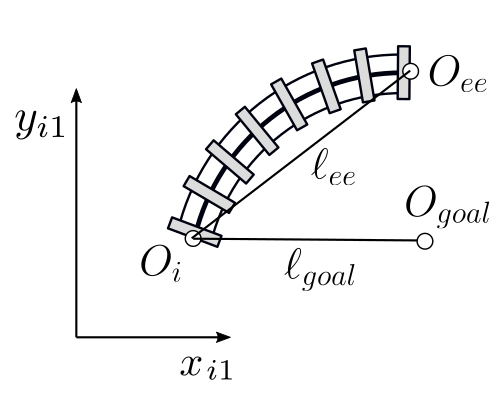
\includegraphics[width=0.6\textwidth]{images/pid_controller.png}
    \caption{Prismatic PID model diagram}
    \label{fig:pid_controller}
\end{figure}

An error term (Equation \eqref{eq:pid/error}) is defined by subtracting the distance between the goal point and an arm's base, and the end effector position and an arm's base. This error is used in a PID controller to yield the joint velocity command in Equation \eqref{eq:pid/complete}. The gains found to result in desirable behaviour are $K_p = 4, K_d = 0, K_i = 0$. 

\begin{align}
    e_i(t) &= ||O_{goal} - O_i|| - ||O_{ee} - O_i|| \label{eq:pid/error}\\
        &= \ell_{goal} - \ell_{ee} \nonumber\\
    \dot q_i &= K_pe_i(t) + K_d \frac{de_i}{dt} + \int e_i(t)dt\label{eq:pid/complete}
\end{align}

This controller has a closed form update, suggesting a computational advantage over the differential constant curvature model which must be solved iteratively. It also is significantly easier to derive and implement in software, making it a fast and easy option for controlling this robot. Because the model does not solve for a curvature value, the robot model is not required. The conversion to motor velocities is handled in the controller gains. 